\documentclass[
  bibliography=totoc,     % Literatur im Inhaltsverzeichnis
  captions=tableheading,  % Tabellenüberschriften
  titlepage=firstiscover, % Titelseite ist Deckblatt
]{scrartcl}

% Paket float verbessern
\usepackage{scrhack}

% Warnung, falls nochmal kompiliert werden muss
\usepackage[aux]{rerunfilecheck}

% deutsche Spracheinstellungen
\usepackage{polyglossia}
\setmainlanguage{german}

% unverzichtbare Mathe-Befehle
\usepackage{amsmath}
% viele Mathe-Symbole
\usepackage{amssymb}
% Erweiterungen für amsmath
\usepackage{mathtools}

% Fonteinstellungen
\usepackage{fontspec}
% Latin Modern Fonts werden automatisch geladen

\usepackage[
  math-style=ISO,    % ┐
  bold-style=ISO,    % │
  sans-style=italic, % │ ISO-Standard folgen
  nabla=upright,     % │
  partial=upright,   % ┘
  warnings-off={           % ┐
    mathtools-colon,       % │ unnötige Warnungen ausschalten
    mathtools-overbracket, % │
  },                       % ┘
]{unicode-math}

% traditionelle Fonts für Mathematik
\setmathfont{Latin Modern Math}
\setmathfont{XITS Math}[range={scr, bfscr}]
\setmathfont{XITS Math}[range={cal, bfcal}, StylisticSet=1]

% Zahlen und Einheiten
\usepackage[
  locale=DE,                 % deutsche Einstellungen
  separate-uncertainty=true, % immer Fehler mit \pm
  per-mode=reciprocal,       % ^-1 für inverse Einheiten
  output-decimal-marker=.,   % . statt , für Dezimalzahlen
]{siunitx}

% chemische Formeln
\usepackage[
  version=4,
  math-greek=default, % ┐ mit unicode-math zusammenarbeiten
  text-greek=default, % ┘
]{mhchem}

% richtige Anführungszeichen
\usepackage[autostyle]{csquotes}

% schöne Brüche im Text
\usepackage{xfrac}

% Standardplatzierung für Floats einstellen
\usepackage{float}
\floatplacement{figure}{htbp}
\floatplacement{table}{htbp}

% Floats innerhalb einer Section halten
\usepackage[
  section, % Floats innerhalb der Section halten
  below,   % unterhalb der Section aber auf der selben Seite ist ok
]{placeins}

% Seite drehen für breite Tabellen
\usepackage{pdflscape}

% Captions schöner machen.
\usepackage[
  labelfont=bf,        % Tabelle x: Abbildung y: ist jetzt fett
  font=small,          % Schrift etwas kleiner als Dokument
  width=0.9\textwidth, % maximale Breite einer Caption schmaler
]{caption}
% subfigure, subtable, subref
\usepackage{subcaption}

% Grafiken können eingebunden werden
\usepackage{graphicx}
% größere Variation von Dateinamen möglich
\usepackage{grffile}

% schöne Tabellen
\usepackage{booktabs}

% Verbesserungen am Schriftbild
\usepackage{microtype}

% Literaturverzeichnis
\usepackage[
  backend=biber,
]{biblatex}
% Quellendatenbank
\addbibresource{lit.bib}
\addbibresource{programme.bib}

% Hyperlinks im Dokument
\usepackage[
  unicode,        % Unicode in PDF-Attributen erlauben
  pdfusetitle,    % Titel, Autoren und Datum als PDF-Attribute
  pdfcreator={},  % ┐ PDF-Attribute säubern
  pdfproducer={}, % ┘
]{hyperref}
% erweiterte Bookmarks im PDF
\usepackage{bookmark}

% Trennung von Wörtern mit Strichen
\usepackage[shortcuts]{extdash}

\author{
  Timo Gräßer
  \texorpdfstring{
    \\
    \href{mailto:timo.graesser@udo.edu}{timo.graesser@udo.edu}
  }{}%
  \texorpdfstring{\and}{, }
  Jasper Karl Lammering%
  \texorpdfstring{
    \\
    \href{mailto:jasper.lammering@udo.edu}{jasper.lammering@udo.edu}
  }{}%
}
\publishers{TU Dortmund – Fakultät Physik}


\subject{V301}
\title{Leerlaufspannung und Innenwiderstand von Spannungsquellen}
\date{
  Durchführung: 10.11.2015
  \hspace{3em}
  Abgabe: 17.11.2015
}

\begin{document}

\maketitle
\thispagestyle{empty}
\tableofcontents
\newpage

\section{Einleitung}
Im folgenden Protokoll bestimmen wir die Leerlaufspannung und den Innenwiderstand
verschiedener Spannungsquellen.

\section{Theorie}
\label{sec:Theorie}

Eine Spannungsquelle ist ein elektrisches Bauteil, dass über einen Zeitraum, der endlich ist,
eine konstante Leistung liefert.

Die Spannung, die an den Ausgängen der Spannungsquelle abgegriffen wird, wird
mit Klemmenspannung $U_\text{K}$ bezeichnet. Wenn kein Strom entnommen wird, bezeichnet
man sie mit Leerlaufspannung $U_\text{0}$. Sobald nun aber ein Stromverbraucher
angeschlossen wird, sinkt $U_K$ auf einen Wert unterhalb $U_\text{0}$ nach der Gleichung
\eqref{eqn:Klemmenspannung}.

\begin{equation}
  U_\text{K}(I) = U_\text{0} - I \cdot R_\text{i}
  \label{eqn:Klemmenspannung}
\end{equation}

Jede Spannungsquelle besitzt einen Innenwiderstand $R_\text{i}$, der bewirkt, dass
ihr keine unendliche Leistung entnommen werden kann.

\begin{equation}
  N = I^2 \cdot R_\text{a}
  \label{eqn:Leistung}
\end{equation}

Mit Gleichung \eqref{eqn:Leistung} kann die Leistung $N$ in Abhängigkeit von der Stromstärke $I$
und dem äußeren Widerstand $R_\text{a}$ berechnet werden.

Wenn man nun aber Gleichung
\eqref{eqn:Klemmenspannung} nach $I$ umformt und in \eqref{eqn:Leistung} einsetzt
zeigt sich, dass die Leistung nur noch von $R_\text{a}$ abhängt nach Gleichung
\eqref{eqn:Leistungmitra}.

\begin{equation}
  N = \frac{(U_\text{0})^2}{(R_\text{i} + R_\text{a})^2} \cdot R_\text{a}
  \label{eqn:Leistungmitra}
\end{equation}

Diese Funktion $N(R_\text{a})$ duchläuft ein Maximum, wie sich in Abbildung
\ref{fig:U5} zeigt. An dieser Stelle spricht man von Leistungsanpassung.

Außerdem muss noch erwähnt werden, dass der Innenwiderstand bei elektrischen
Generatoren durch Gleichung \eqref{eqn:Innenwiderstand} ausgedrückt wird.

\begin{equation}
  R_\text{i} = \frac{\text{d}U_\text{K}}{\text{d}I}
  \label{eqn:Innenwiderstand}
\end{equation}

\newpage

\section{Durchführung}
\label{sec:Durchführung}

\begin{enumerate}
  \item  Es wird die Leerlaufspannung der Monozelle unmittelbar gemessen und
  der angegebene Eingangswiderstand $R_\text{V}$ notiert.

  \item  Die Klemmenspannung $U_\text{K}$ wird bei variablem Belastungsstrom $I$
  aufgenommen. Im Einzelnen werden 10 Messwertpaare aufgenommen.
  Um den Strom zu variieren wird  der Belastungswiderstand variiert.
  Das geschah durch Variation des variablen Widerstands im Bereich von 0-\SI{50}{\Omega}.
  Dazu wurde die Schaltung aus Abbildung \ref{fig:Schaltung1} verwendet.

\begin{figure}[h]
  \centering
  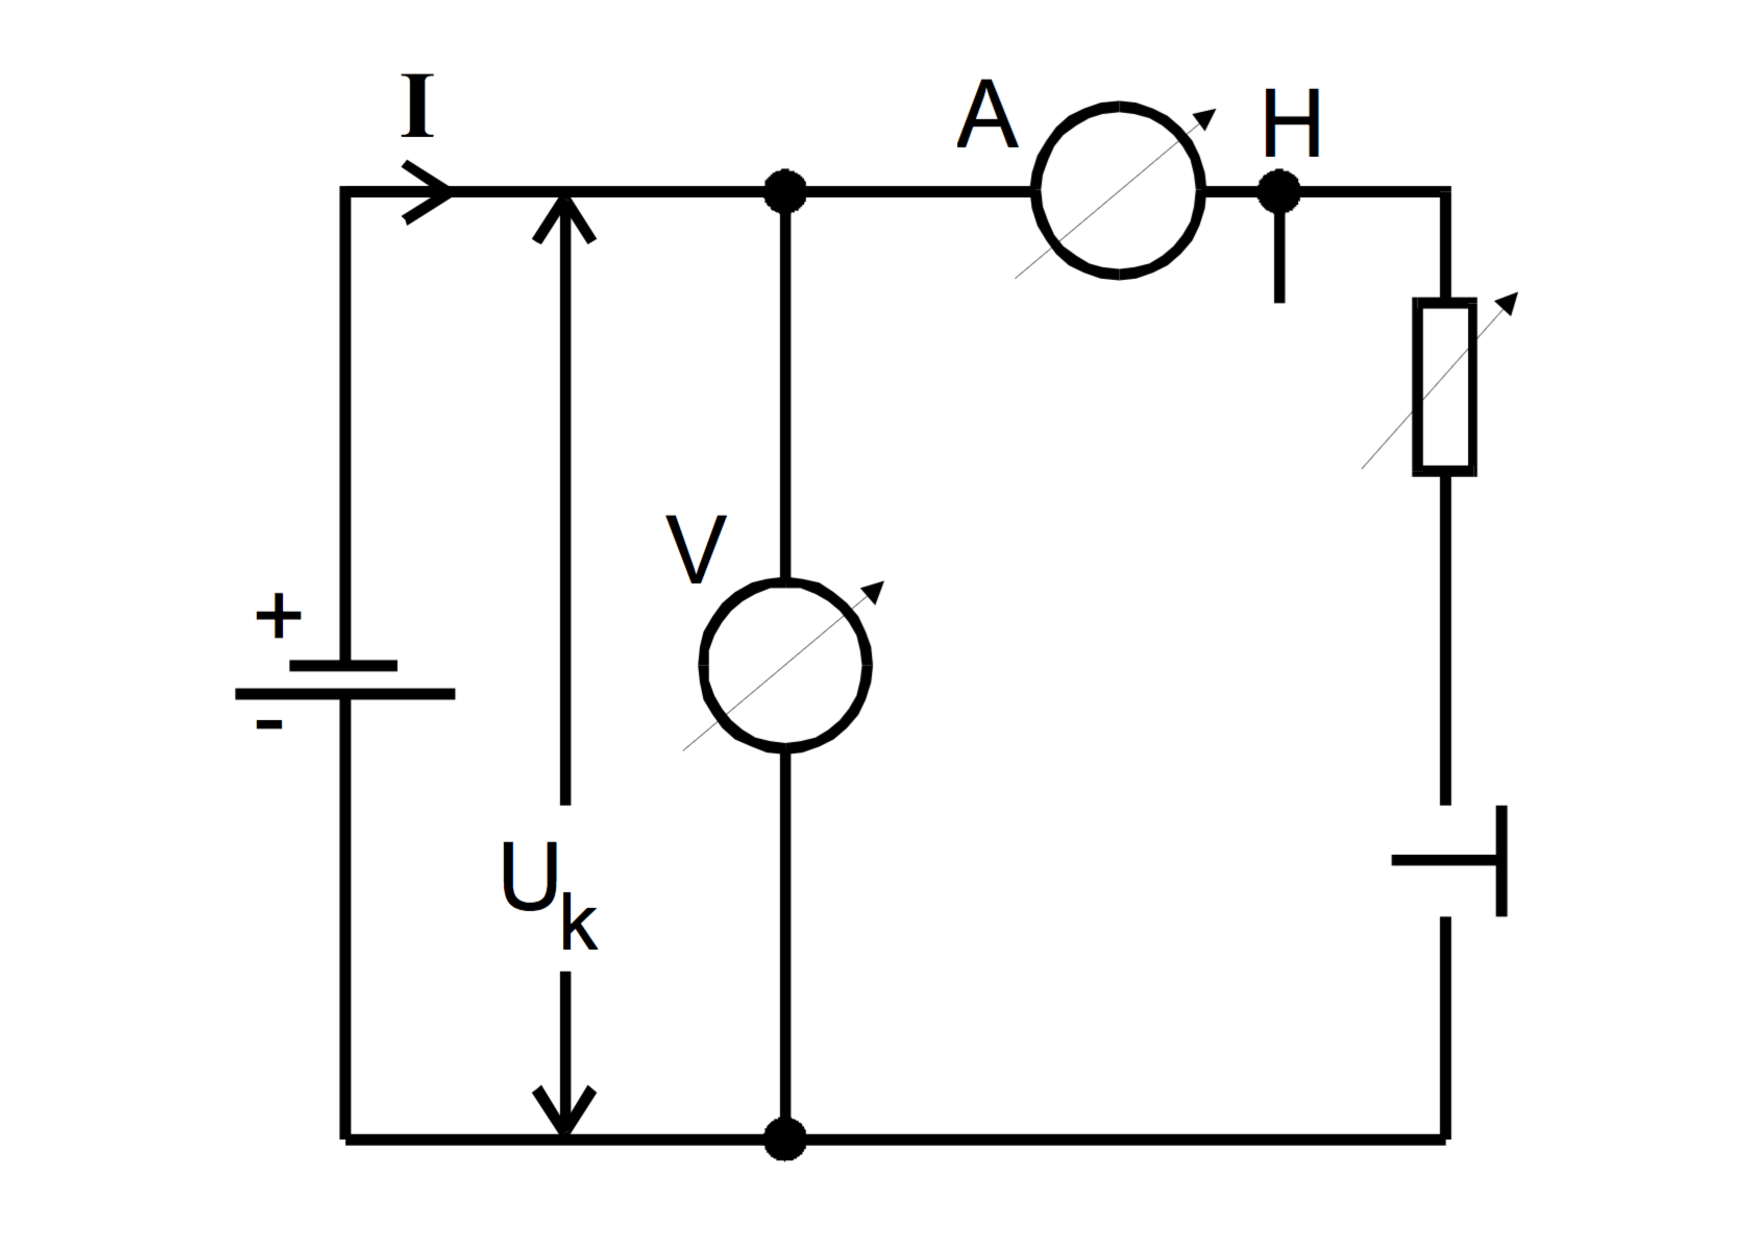
\includegraphics[height = 5cm]{Abbildung 1.pdf}
  \caption{Messschaltung 1 zum Messen an der Monozelle.\cite{anleitung}}
  \label{fig:Schaltung1}
\end{figure}

  \item Dann wird eine Gegenspannung in die Schaltung eingebaut, die den Strom
  in die entgegengesetzte Richtung fließen lässt, da sie ca. \SI{2}{\volt} größer
  ist als $U_{\text{0}}$. Hier ändert sich die Klemmenspannung
  wie in Gleichung \eqref{eqn:Gegenspannung}.

\begin{equation}
  U_\text{K} = U_\text{0} + IR_\text{i}
  \label{eqn:Gegenspannung}
\end{equation}

  Es wurden aber erneut $U_\text{K}$ und $I$ aufgenommen. Das geschah bei
  Variation des Widerstands im selben Bereich wie in Schritt 2. Es werden
  erneut 10 Messwertpaare notiert. Abbildung \ref{fig:Schaltung2}
  zeigt die verwendete Schaltung.

\begin{figure}[h]
  \centering
  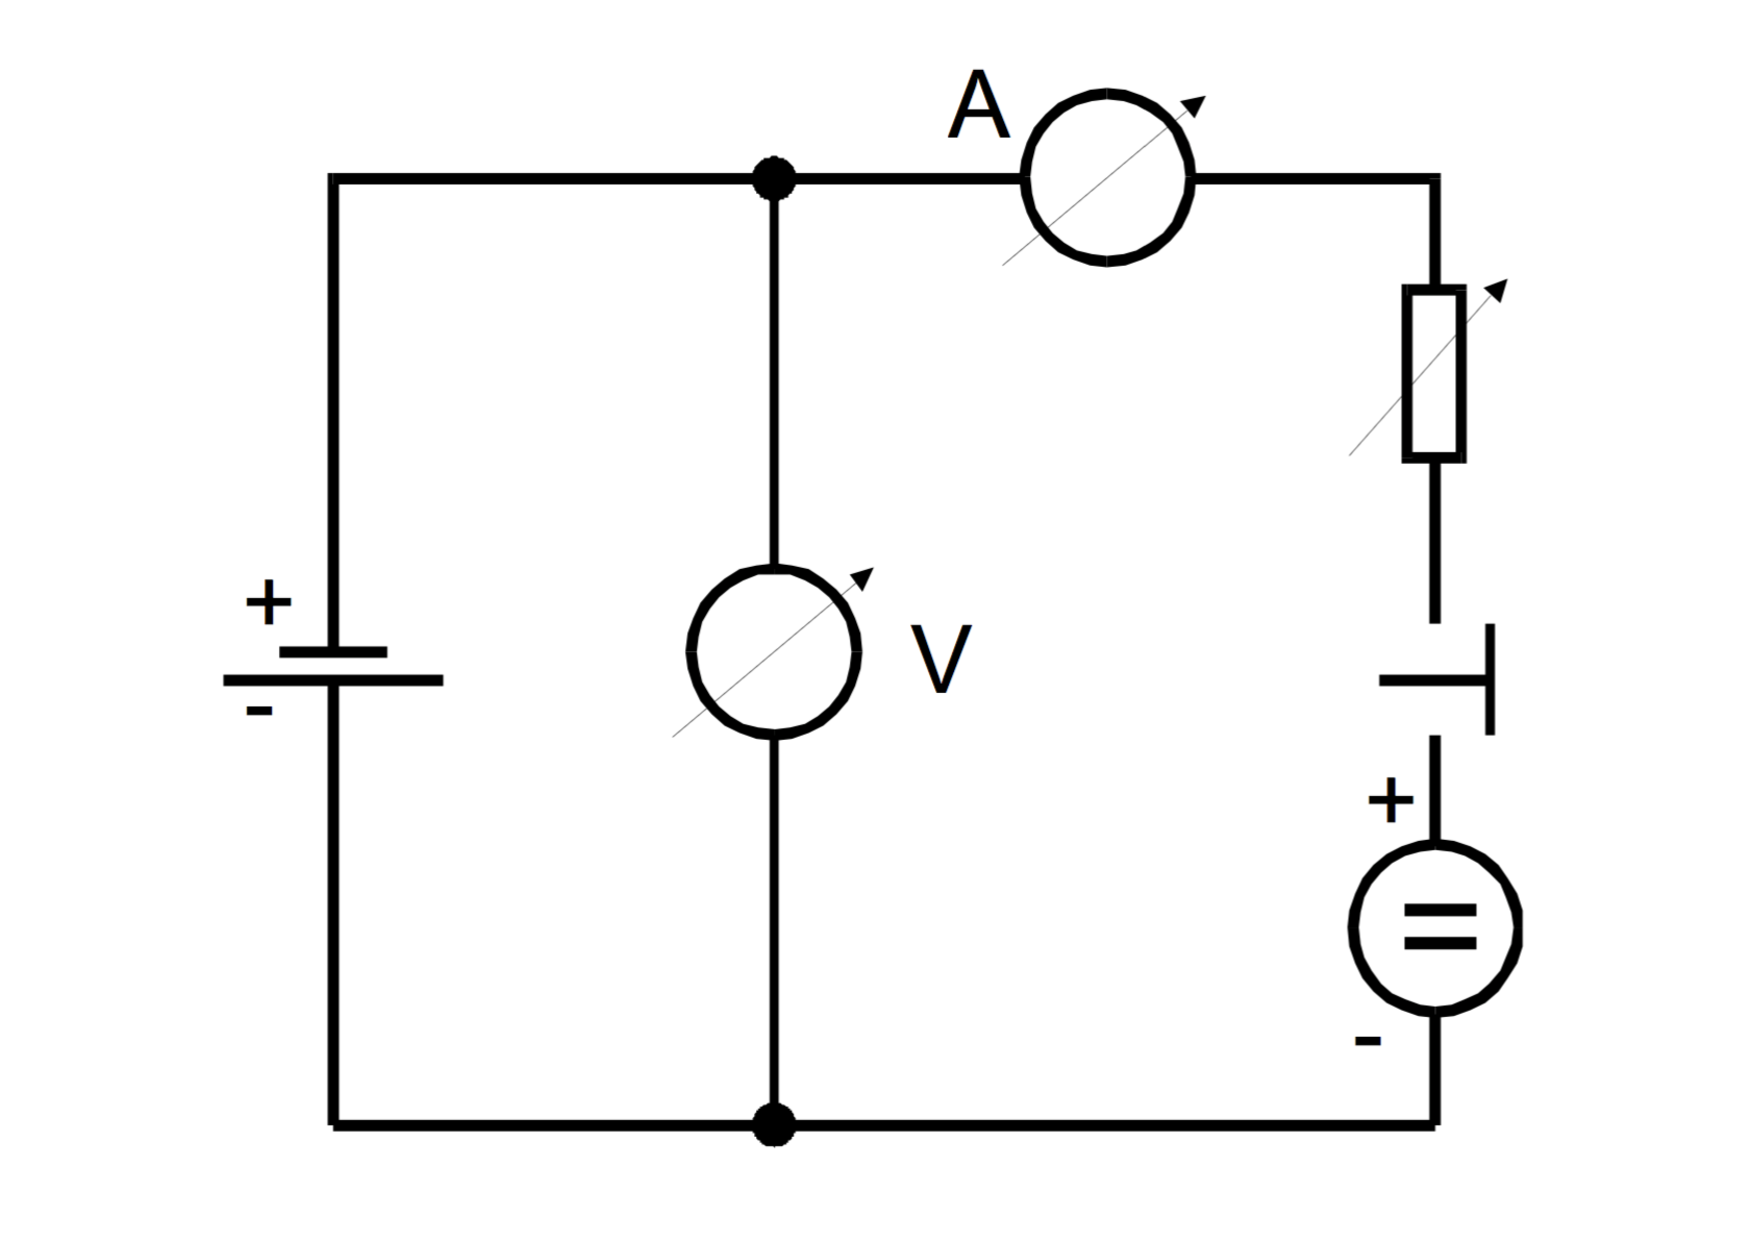
\includegraphics[height = 5cm]{Abbildung 2.pdf}
  \caption{Messschaltung 2 mit der Gegenspannung.\cite{anleitung}}
  \label{fig:Schaltung2}
\end{figure}

  \item Zuletzt wird die Messung aus Schritt 2 widerholt; allerdings mit dem Sinus-
  und Rechteckausgang eines RC-Generators als Messobjekt. $R_\text{a}$ wird für
  den \SI{1}{\volt}-Sinusausgang im Bereich von 20 bis \SI{250}{\Omega} und für den
  \SI{1}{\volt}-Rechteckausgang im Bereich von 0.1 bis \SI{5}{\kilo\Omega} variiert.
  Die Schaltungen mit dem Rechteck- und Sinusausgang als Messobjekte werden im
  Folgenden mit 3a beziehungsweise mit 3b bezeichnet. Sie sind analog zu Abbildung
  \ref{fig:Schaltung1} nur dass an Stelle der Gleichstromquelle der $RC$-Generator
  angeschlossen wird.
\end{enumerate}

\input{Praeambel.tex}
\begin{document}
  \section{Auswertung}
  \subsection{Messergebnisse}

  In den Tabellen \ref{tab:U1} und \ref{tab:U2} sind jeweils
  Klemmenspannung $U_k$ und Stromstärke $I$
  der ersten und zweiten Schaltung aufgetragen. Der Belastungswiderstand $R_A$
  lag im Bereich $ \SI{0}{\ohm} \leq R_A \leq \SI{50}{\ohm} $.
  Die Messfehler betrugen für beide Messungen $U_\text{k,m} = \SI{+-0.06}{\V}$
  und $I_m = \pm \SI{0.003}{\A}$.
  Es ist zu beachten, dass die ersten beiden Werte der Stromstärke bei
  der ersten Messung und die ersten drei Werte der Stromstärke bei der zweiten
  Messung einen 10-mal so großen Messfehler haben.

  \begin{table}[h]
    \begin{minipage}{0.45\textwidth}
    \centering
    \begin{tabular}{S S}
      \toprule
      $U_k/\si{\V}$ & $I/\si{\A}$ \\
      \midrule
      0.60 & 0.230 \\
      0.70 & 0.140 \\
      0.93 & 0.086 \\
      1.05 & 0.065 \\
      1.13 & 0.052 \\
      1.16 & 0.045 \\
      1.21 & 0.038 \\
      1.22 & 0.034 \\
      1.25 & 0.030 \\
      1.26 & 0.028 \\
      \bottomrule
    \end{tabular}
    \label{tab:U1}
    \caption{Messwerte von Schaltung 1}
    \end{minipage}\hfill
    \begin{minipage}{0.45\textwidth}
      \centering
      \begin{tabular}{S S}
        \toprule
        $U_k/\si{\V}$ & $I/\si{\A}$ \\
        \midrule
        3.25 & 0.330 \\
        2.49 & 0.185 \\
        2.17 & 0.122 \\
        1.99 & 0.096 \\
        1.88 & 0.075 \\
        1.80 & 0.062 \\
        1.76 & 0.054 \\
        1.73 & 0.048 \\
        1.69 & 0.042 \\
        1.67 & 0.038 \\
        \bottomrule
      \end{tabular}
      \label{tab:U2}
      \caption{Messwerte von Schaltung 2}
    \end{minipage}
  \end{table}

  Bei der ersten Messung der Leerlaufspannung der Monozelle betrug die
  gemessene Klemmenspannung
  \begin{equation}
    U_\text{k,0} = \SI{1.40(6)}{\V}.
  \end{equation}
  Der Eingangswiderstand $R_V$ des Voltmeters ist
  \begin{equation}
    R_V = \SI{10}{\mega\ohm}
  \end{equation}
  Zur lineare Ausgleichsrechnung wurde die Funktion linregress aus scipy.stats
  benutzt. Es wurde jeweils Steigung, Y-Achsen-Abschnitt und die
  Messungenauigkeit zurückgegeben.

  \newpage

  \begin{figure}[h]
    \includegraphics[width = \textwidth]{plot1.pdf}
    \label{fig:U1}
    \caption{Messwerte und Fehler $U_\text{k,1}(I)$}
  \end{figure}

  In dem Graphen \ref{fig:U1} sind die Messwerte der Tabelle
  \ref{tab:U1} und ihre lineare Regression
  $U_\text{k,1}(I)$ aufgetragen.
  Das erste Wertepaar $\SI{0.60}{\V}/ \SI{0.230}{\A}$
  wurde allerdings nicht mit in den Plot einbezogen,
  da es sehr stark von den anderen Wertepaaren abweicht und
  den Messfehler der linearen Regression stark vergrößert.
  Folgende Werte wurden bei der Ausgleichsrechnung zurückgegeben:
  \begin{align}
    m_1 & = \num{-0.196 +- 0.005} & b_1 & = 0.273
  \end{align}
  Mit
  \begin{equation}
    U_\text{k,1}(I) = U_\text{0,1} - I \cdot R_\text{i,1}
  \end{equation}
  für die erste Schaltung ist
  \begin{equation}
    U_\text{0,1} = b_1 \si{\V} = \SI{0.273}{\V}
  \end{equation}
  und
  \begin{equation}
    R_\text{i,1} = -m_1 \si{\ohm} = \SI{0.196 +- 0.005}{\ohm}.
  \end{equation}

  \newpage

  \begin{figure}[h]
    \includegraphics[width = \textwidth]{plot2.pdf}
    \label{fig:U2}
    \caption{Messwerte und Fehler $U_\text{k,2}(I)$}
  \end{figure}

  In dem Graphen \ref{fig:U2} sind die Messwerte der Tabelle
  \ref{tab:U2} und ihre lineare Regression
  $U_\text{k,2}(I)$ aufgetragen.
  Bei der Ausgleichungsrechnung wuden folgene Werte zurückgegeben:
  \begin{align}
    m_2 & = \num{5.44 +- 0.06} & b_2 & = 1.47
  \end{align}
  Da in Schaltung 2 eine Gegenspannung, die in etwa $\SI{2}{\V}$ größer als
  $U_0$ ist, mit eingebaut wurde, fließt der Strom in umgekehrte Richtung.
  Die Klemmenspannung ist daher
  \begin{equation}
    U_\text{k,2}(I) = U_\text{0,2} + I \cdot R_\text{i,2}.
  \end{equation}
  Für Schaltung 2 ergeben sich dann Leerlaufspannung
  \begin{equation}
    U_\text{0,2} = b_2 \si{\V} = \SI{1.47}{\V}
  \end{equation}
  und Innenwiderstand
  \begin{equation}
    R_\text{i,2} = m_2 \si{\ohm} = \SI{5.44 +- 0.06}{\ohm}.
  \end{equation}

  \newpage

  In den Tabellen \ref{tab:U3a} und \ref{tab:U3b} sind jeweils
  Klemmenspannung $U_K$ und Stromstärke $I$
  der Schaltungen 3a und 3b aufgetragen. Der Belastungswiderstand $R_A$
  lag bei 3a im Bereich $ \SI{20}{\ohm} \leq R_A \leq \SI{250}{\ohm} $ und bei
  3b im Bereich $ \SI{0.1}{\kilo\ohm} \leq R_A \leq \SI{5}{\kilo\ohm} $ .
  Die Messfehler beim Rechteck-Ausgang 3a betrugen
  $U_\text{k,m} = \SI{+-0.03}{\V}$ und $I_m = \pm \SI{0.3}{\milli\A}$ und die
  beim Sinus-Ausgang 3b $U_\text{k,m} = \SI{+-0.09}{\V}$ und
  $I_m = \pm \SI{0.09}{\milli\A}$.

  \begin{table}[h]
    \begin{minipage}{0.45\textwidth}
    \centering
    \begin{tabular}{S S}
      \toprule
      $U_k/\si{\V}$ & $I/\si{\milli\A}$ \\
      \midrule
      0.165 & 6.4 \\
      0.215 & 5.5 \\
      0.275 & 4.3 \\
      0.318 & 3.5 \\
      0.341 & 3.0 \\
      0.361 & 2.6 \\
      0.378 & 2.3 \\
      0.393 & 2.1 \\
      0.403 & 1.9 \\
      0.412 & 1.7 \\
      \bottomrule
    \end{tabular}
    \label{tab:U3a}
    \caption{Messwerte von Schaltung 1}
    \end{minipage}\hfill
    \begin{minipage}{0.45\textwidth}
      \centering
      \begin{tabular}{S S}
        \toprule
        $U_k/\si{\V}$ & $I/\si{\milli\A}$ \\
        \midrule
        0.73 & 2.55 \\
        1.22 & 1.84 \\
        1.55 & 1.26 \\
        1.76 & 0.93 \\
        1.89 & 0.71 \\
        1.96 & 0.59 \\
        2.01 & 0.50 \\
        2.06 & 0.45 \\
        2.08 & 0.41 \\
        2.10 & 0.37 \\
        \bottomrule
      \end{tabular}
      \label{tab:U3b}
      \caption{Messwerte von Schaltung 2}
    \end{minipage}
  \end{table}

  \newpage

  \begin{figure}[h]
    \includegraphics[width = \textwidth]{plot3a.pdf}
    \label{fig:U3a}
    \caption{Messwerte und Fehler $U_\text{k,3a}(I)$}
  \end{figure}

  In dem Graphen \ref{fig:U3a} sind die Messwerte der Tabelle
  \ref{tab:U3a} und ihre lineare Regression
  $U_\text{k,3a}(I)$ aufgetragen.
  Folgende Werte wurden bei der Ausgleichsrechnung ausgegeben:
  \begin{align}
    m_\text{3a} & = \num{-19.1 +- 0.2} & b_\text{3a} & = 9.567
  \end{align}
  Mit
  \begin{equation}
    U_\text{k,3a}(I) = U_\text{0,3a} - I \cdot R_\text{i,3a}
  \end{equation}
  für die erste Schaltung ist
  \begin{equation}
    U_\text{0,3a} = b_\text{3a} \si{\V} = \SI{9.567}{\V}
  \end{equation}
  und
  \begin{equation}
    R_\text{i,3a} = -m_\text{3a} \si{\ohm} = \SI{0.196 +- 0.005}{\ohm}.
  \end{equation}

  \newpage

  \begin{figure}[h]
    \includegraphics[width = \textwidth]{plot3b.pdf}
    \label{fig:U3b}
    \caption{Messwerte und Fehler $U_\text{k,3b}(I)$}
  \end{figure}

  In dem Graphen \ref{fig:U3b} sind die Messwerte der Tabelle
  \ref{tab:U3b} und ihre lineare Regression
  $U_\text{k,3b}(I)$ aufgetragen.
  Folgende Werte wurden bei der Ausgleichsrechnung ausgegeben (umgerechnet von
  \si{\milli\A} in \si{\A}):
  \begin{align}
    m_\text{3b} & = \num{-621(6)e2} & b_\text{3b} & = 2.333
  \end{align}
  Mit
  \begin{equation}
    U_\text{k,3b}(I) = U_\text{0,3b} - I \cdot R_\text{i,3b}
  \end{equation}
  für die erste Schaltung ist
  \begin{equation}
    U_\text{0,3b} = b_\text{3b} \si{\V} = \SI{2.333}{\V}
  \end{equation}
  und
  \begin{equation}
    R_\text{i,3b} = -m_\text{3b} \si{\ohm} = \SI{-621(6)e2}{\ohm}.
  \end{equation}

  \newpage

  Bei der Messung der Leerlaufspannung $U_0$ mit einem hochohmigen Voltmeter
  wurde der Vorteil ausgenutzt, dass bei einer niedrige Stromstärke die
  gemessene Klemmenspanung $U_k$ etwa der Leerlaufspannung entspricht, da
  der Anteil des Innenwiderstandes nahe Null ist.
  Es existiert dennoch ein geringer Fehler, der im Folgenden bestimmt wird.
  Mit
  \begin{equation}
    I = \frac{U_\text{k,0}}{R_V} = \SI{1.40(6)e-7}{\A}
  \end{equation}
  und dem in \ref{fig:U1} bestimmten Innenwiderstand
  \begin{equation}
    R_\text{i,1} = \SI{0.196 +- 0.005}{\ohm}
  \end{equation}
  ergibt sich der systematische Fehler ohne Abweichung mit der Formel
  \begin{equation}
    U_\text{0,0} - U_\text{k,0} = I \cdot R_i = \num{0.2744e-7} \si{\V}
  \end{equation}
  Für die Bestimmung der Abweichung muss die Messfehlerfortpflanzung
  beachtet werden. Über die Formel zur Gaußschen Fehlerfortpflanzung
  \begin{equation}
    \phi = \sqrt{\sum_{i=1}^{N} \biggl(\frac{\partial f}{\partial x_i}\biggr)^2
    \cdot \sigma_i^2}
  \end{equation}
  ergibt sich die neue Abweichung
  \begin{equation}
    \phi = \sqrt{\frac{\partial(I \cdot R_i)}{\partial I} \cdot \sigma_I^2
    + \frac{\partial(I \cdot R_i)}{\partial R_i} \cdot \sigma_\text{R}^2}
    = 1.8708 \cdot 10^{-6}
  \end{equation}
  Die Leerlaufspannung $U_\text{0,0}$ mit systematischem Fehler und der
  resultierenden Abweichung beträgt dann
  \begin{equation}
    U_\text{0,0} = \SI{1400000(2)e-6}{\V}.
  \end{equation}

  Wenn man in der Schaltung 1 das Voltmeter an die Stelle H
  setzen würde, würden die Messwerte der Klemmenspannung $U_k$ und der
  Stromstärke $I$ verfälscht werden. Das Voltmeter hat zwar einen großen
  Widerstand $R_V = \SI{10}{\mega\ohm}$, aber dennoch fließt ein kleiner Strom
  über diesen Pfad. Das Amperemeter würde also die Summe aus dem
  Klemmen-Strom $I_k$ und dem Voltmeter-Strom $I_V$ messen und nicht einfach
  nur den gesuchten Klemmen-Strom $I_k$.
  Zudem misst das Voltmeter nur die Potentialdifferenz an dem Außenwiderstand
  $R_A$ und nicht zusätzlich die minimale Spannung am Amperemeter. Dadurch
  sind die Werte des Innenwiderstandes $R_I$ ebenfalls verfälscht.
\end{document}

\section{Diskussion}
\label{sec:Diskussion}

Wenn man in der Schaltung \ref{fig:Schaltung1} das Voltmeter an die Stelle H
setzen würde, würden die Messwerte der Klemmenspannung $U_k$ und der
Stromstärke $I$ verfälscht werden. Das Voltmeter hat zwar einen großen
Widerstand $R_V = \SI{10}{\mega\ohm}$, aber dennoch fließt ein kleiner Strom
über diesen Pfad. Das Amperemeter würde also die Summe aus dem
Klemmen-Strom $I_k$ und dem Voltmeter-Strom $I_V$ messen und nicht einfach
nur den gesuchten Klemmen-Strom $I_k$.
Zudem misst das Voltmeter nur die Potentialdifferenz an dem Außenwiderstand
$R_A$ und nicht zusätzlich die minimale Spannung am Amperemeter. Dadurch
sind die Werte des Innenwiderstandes $R_I$ ebenfalls verfälscht.


\nocite{anleitung}

\printbibliography

\newpage

\appendix

\section{Kopie der Originaldateien}

\end{document}
